%\documentclass[10pt,twocolumn,letterpaper]{article}
\documentclass{llncs}
\usepackage{subfigure}
%\usepackage[margin=1in]{geometry}
%\usepackage{palatino}
\usepackage{listings}
\usepackage[sort]{cite}
\usepackage{framed}
\usepackage{enumitem}
%\usepackage[small]{titlesec}
\usepackage[usenames,dvipsnames,svgnames,table]{xcolor}
\usepackage[framemethod=tikz]{mdframed}
\usepackage{color}
\usepackage{minted}
\PassOptionsToPackage{hyphens}{url}\usepackage{hyperref}

%\newcommand{\elaine}[1]{{\color{red}{[elaine: #1]}}}
\newcommand{\elaine}[1]{}
\newcommand{\anote}[1]{{\color{magenta}{[AM: #1]}}}
\newcommand{\ignore}[1]{}

\renewcommand{\paragraph}[1]{\vspace{5pt} \noindent{\bf #1}}


\lstset{
	tabsize = 4
}

\begin{document}
%\title{A Smart Contract Programming Lab: Lessons and Insights}
\title{Step by Step Towards Creating a Safe Smart Contract: Lessons and Insights from a Cryptocurrency Lab}

\author{
%  Kevin Delmolino\\
% \texttt{del@terpmail.umd.edu}
%  \and
%  Mitchell Arnett\\
%  \texttt{marnett@umd.edu}
%  \and
%  Ahmed Kosba\\
%  \texttt{akosba@cs.umd.edu}
% \and
%  Andrew Miller\\
%  \texttt{amiller@cs.umd.edu}
%  \and
%  Elaine Shi\\
%  \texttt{runting@gmail.com}
}

\date{}
\maketitle

%\setcounter{tocdepth}{5}
%\tableofcontents

%\newpage
\begin{abstract}
We document our experiences in teaching smart contract 
programming to undergraduate students at the University of [anonymized for submission],
the first pedagogical attempt of its kind.
Since smart contracts deal directly with the movement of valuable currency units
between contratual parties, 
security of a contract program is of paramount importance.  

Our lab exposed numerous common pitfalls 
in designing safe and secure smart contracts. 
We document several typical classes of mistakes students made, %reflect on them, 
suggest ways to fix/avoid them, 
and advocate best practices for programming smart contracts.
Finally, our pedagogical efforts have also resulted in online open
course materials for 
programming smart contracts, which may be of indepdendent interest to the community.
\end{abstract}

\section{Introduction}

%\elaine{rewrite}
Completely decentralized cryptocurrencies like Bitcoin~\cite{satoshi-bitcoin}
and other altcoins~\cite{altcoins}
have captured the public's attention and interest, 
and have been much more successful than any prior incarnations of electronic
cash. Many would call the rise 
of these electronic currencies a technological revolution, and the ``wave of
the future''~\cite{riseandrise}.
Emerging altcoins such as Ethereum~\cite{ethereum} and Counterparty~\cite{counterparty}
extend Bitcoin's design by offering a rich programming language for 
writing ``smart contracts.'' Smart
contracts are user-defined programs that specify rules 
governing transactions, and that are enforced by
the network of peers (assuming the underlying cryptocurrency is secure). 
In comparison with traditional
financial contracts, smart contracts carry the promise of low legal 
and transaction costs, and can 
lower the bar of entry for users.

In Fall 2014, at the University of [anonymized], 
we organized a new, hands-on
smart contract programming lab in 
our undergraduate-level security
%``CMSC 414: Computer and Network Security'' 
%our undergraduate security
class -- the first of its
kind that has ever been attempted.


%Cryptocurrencies, including Bitcoin, Ethereum, and many others, are an exciting new technology. They are experimental distributed systems that allow users to manipulate virtual currency. Actual stored wealth and monetary value are at stake! Ethereum is the first embodiment of the more general idea: it provides an expressive and flexible programming environment for controlling and interacting with money.

%This tutorial is intended for instructors
%who wish to conduct a smart  
%contract programming lab, or students/developers
%who want to learn about smart contract programming.

\ignore{
The first part of this lab consists of step-by-step examples illustrating basic design of functional smart contracts. We highly recommend you take a hands-on approach, and interact with these smart contract examples using the Ethereum simulator! The accompanying materials to everything you need to get started with experimenting, including  a virtual machine image, basic instructions, and a language guide.

The second part of this lab focuses on designing smart contracts that achieve their intended goals, and are robust to attacks. 
Although our lab makes us of a simulator, the smart contracts you write can also be used in the live Ethereum network\footnote{At the time of this writing, the only live Ethereum network is a test network, since the main network has not yet launched.} The basic concepts we discuss apply to other cryptocurrencies as well (including Bitcoin), so most of what you learn will be transferable.
}

\paragraph{Smart contract programming: unique challenges.}
Although smart contract programming in many ways resembles 
traditional programming, 
it raises important new security challenges. 
%Smart contract design is inherently security-oriented. 
Contracts are ``play-for-keeps'', since virtual currencies have real value. 
If you load money into a buggy smart contract, you will likely lose it. 
Further, smart contract programming requires
an ``economic thinking'' perspective that traditional
programmers may not have acquired.
Contracts must be written to ensure fairness even when
counterparties may be incentivized to cheat in arbitrary ways to maximize
their economic gains.

%\elaine{say more about all parties being 
%selfish, and may do malicious things to maximize its
%financial gains.} 

%\elaine{stress that even programming a very simple
%game like rock paper scissors was difficult
%and exposed many problems.}


As an outcome of our lab, we observed several classes
of typical mistakes students made. 
%While bugs such as buffer overflows are 
%typical of 
In contrast to  
traditional software development where 
bugs such as buffer overflows are typical, 
in our lab, we observed 
bugs and pitfalls that arise due to 
%Several of such mistakes 
%are specific to 
the unique nature of smart contract programs.
%may not be observa
%These mistakes suggest that programming safe smart contracts 
%is difficult. 

Our lab experiences show that even for 
very simple smart contracts (e.g., a 
``Rock, Paper, Scissors'' game), 
designing and implementing them correctly
was highly non-trivial.
%The students' programs exhibited several classes
%of common pitfalls, suggesting that 
This suggests that extra precautions 
and scrutiny 
are necessary when programming smart contracts.

In this paper, although we adopt Ethereum's Serpent language,
most of the the insights we gain 
are not language-specific, but can be generalized to 
smart contract programming
under a broad model.


\paragraph{Open-source course and lab materials.}
Based on lessons and insights 
drawn through this experimental lab, we have designed
new, open course materials and lab designs 
for smart contract programming~\cite{anonymousethlab}.
We hope that these open-source course materials and labs
will aid both instructors who 
wish to teach smart contract programming and students/developers who 
wish to teach themselves smart contract programming.
\elaine{probably the langugage can be better.}

\paragraph{Broader insights gained.}
Inspired by our experimental 
smart contract lab, 
we argue why cryptocurrency and smart contracts 
will serve as a great pedagogical platform 
for Cybersecurity education.
We also draw from our experiences
why the ``build, break, and amend your own program'' 
approach is beneficial to instructing adversarial thinking
and incentivizing a student-driven learning 
atmosphere.

\paragraph{Roadmap.}
In the remainder of this paper, we will first give more background on 
cryptocurrency and smart contracts (Section \ref{sec:Background}). 
We will then detail experiences with our lab (Section \ref{sec:lab}),  
the typical pitfalls we observed in smart  
contract programming (Section \ref{sec:pitfalls}), 
and the insights and lessons learned. 



%In a decentralized cryptocurrency like Ethereum, smart contract programs
%are propagated to the entire network, and therefore
%security through obscurity  
%Unlike other hands-on labs in cryptography (e.g., sending encrypted emails with GPG), where actual attacks are unlikely or hard to observe, the attackers in a cryptocurrency are much more apparent. (For example, if you publish a Bitcoin transaction with a ``weak'' brainwallet password, it will be stolen within seconds by hackers who have built tables of the most common passwords. 
%\elaine{Cite Joe's Bonneau's paper}
\ignore{
Smart contract design also requires economic thinking. We use a running example about a rock-paper-scissors game. To help keep incentives in focus, we reward the winner with a monetary prize, so both participants have a stake in the outcome.  Other, more clearly “useful” application include derivative financial instruments, for example that allow people to buy or sell insurance against events that can be “logged” by the network, such as the price of another cryptocurrency. Smart contracts can also be used to raise “crowdfunding” money with a Kickstarter-like assurance contract, that gives contributors a refund if a donations target isn’t reached. In all of these applications, we will want to guarantee that the smart contracts are ``fair'' and aren't profitable to exploit.
}
%% For the users' convenience, we offer
%% a VM image with appropriate  
%% versions of the software pre-installed~\cite{vmimage}.
%% We also provide detailed Ethereum reference manuals
%% geared towards this specific 
%% snapshot of Serpent~\cite{serpentref}.
%% Finally, we also recommend the reader
%% to a more concise, Powerpoint presentation of this tutorial
%% by Elaine Shi and Andrew Miller~\cite{Shi2015}.

%, such that when
%rational miners comprise the majority of compute
%power (or other forms of resources),
%in a Nash equilibrium, it is in the best interest
%of rational miners to honestly execute a
%contract's program logic.

\section{Background}
\label{sec:Background}
In this section, we provide some background on cryptocurrencies and the programming model of smart contracts.

\subsection{Background on Decentralized Cryptocurrencies}
%\paragraph{The Underlying Cryptocurrency.}
Smart contracts are built on top of an underlying cryptocurrency platform. A cryptocurrency is a decentralized system for interacting with virtual money in a shared global ledger. Users transfer money and interact with contracts by publishing signed messages called \emph{transactions} to the cryptocurrency network. The network consists of nodes (called miners) who propagate information, store data, and update the data by applying transactions. A high-level schematic is shown in Figure~\ref{fig:schematic}.
\begin{figure}[t]
\centering
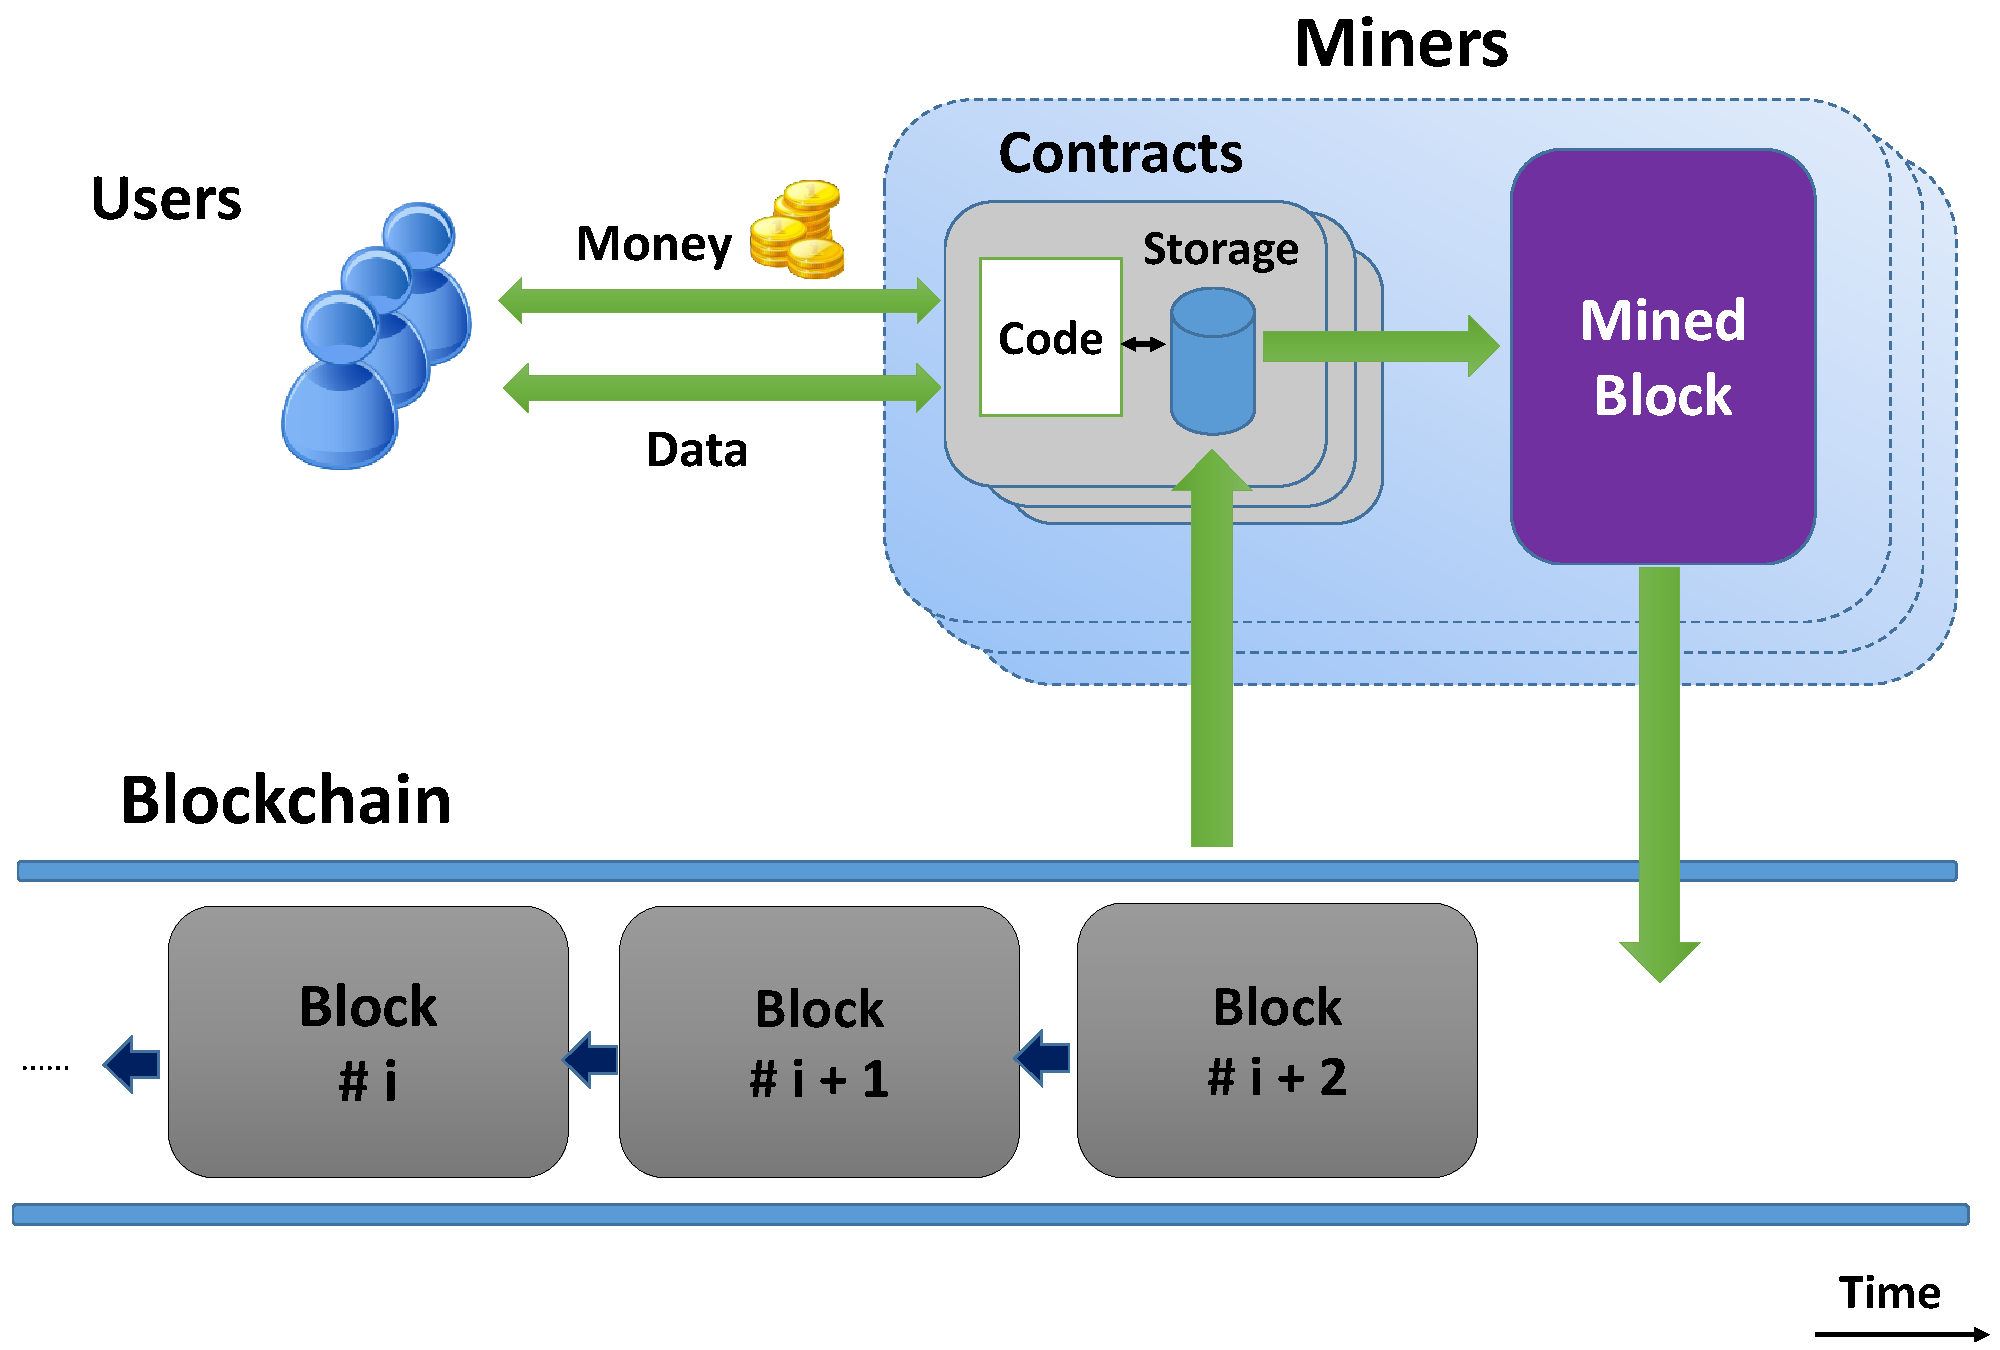
\includegraphics[width=0.7\columnwidth]{overview_figure}
\caption{{\bf Schematic of a decentralized cryptocurrency system 
with smart contracts.}
A smart contract's state is stored on the public blockchain.
A smart contract program is executed by a 
network of miners who reach consensus on the
outcome of the execution, and update the contract's state 
on the blockchain accordingly.
Users can send money or data to a contract;
or receive money or data from a contract.
}
\label{fig:schematic}
\end{figure}

Although the ideas behind cryptocurrencies date back at least twenty-five years (e.g., cryptographic e-cash~\cite{chaum-ecash}), a recent surge of interest in this technology has been incited by the success of Bitcoin~\cite{bitcoin}. For a comprehensive survey on Bitcoin and other cryptocurrencies, see ~\cite{researchperspectives,bittertobetter}.

\ignore{We shall make some simplifying assumptions 
about the security model of the underlying cryptocurrency.
Loosely speaking, we assume that the
cryptocurrency has a secure and incentive compatible
consensus protocol. 
In reality, existing decentralized cryptocurrencies
achieve only heuristic security; designing a provably  
secure decentralized consensus protocol under
rationality assumptions is a topic of 
future research.
}

The main interface provided by the underlying cryptocurrency is an append-only log called a \emph{blockchain}, which imposes a partial or total ordering on transactions submitted by users. The data in the blockchain is guaranteed to be \emph{valid} according to certain predefined rules of the system (e.g., there are no double-spends or invalid signatures). All of the data in the blockchain is public, and every user can access a copy of it. No one can be \emph{prevented} from submitting transactions and getting them included in the blockchain (with at most some small delay). There is global agreement among all nodes and users about the contents of the blockchain,  except for the most recent handful of blocks which have not yet settled.

We also assume that the built-in currency has a stable monetary value. Users have an incentive to gain more of (and avoid losing) units of this currency. Anyone can acquire 
the virtual currency by purchasing or trading for it using 
other fiat currencies (e.g., US dollars) or virtual currencies. The currency is assumed to be fungible; one unit of ether (the currency unit of Ethereum) is exactly as valuable as any other, regardless of the currency's ``history.''

The system keeps track of ``ownership'' of the currency by associating each unit of currency to an ``address''. 
%There are two kinds of addresses: one for users, and one for contracts. 
A user address is a hash of a public key; whoever knows the corresponding private key can spend the money associated to that address. Users can create as many accounts as they want, and the accounts need not be linked to their real identity.

\subsection{Background on Smart Contracts}

\paragraph{Need for general smart contracts.}
Bitcoin offers a rudimentary scripting system
that is neither Turing complete nor user-friendly.
A line of work in both academia and industry 
has attempted to design various smart contract
applications in a way that retrofits Bitcoin's 
scripting language~\cite{iddo-lottery,oakland-lottery,liarcoins,micropay}. 
Due to fundamental limits of the expressiveness of Bitcoin's 
scripting language, 
retrofitting the language
is not only time consuming, but can also result
in asymptotically more costly implementations  
in terms of number of rounds or on-chain cost -- in comparison, many of the same tasks
would be easier to program
and more efficient, if they were built atop a general, Turing-complete
smart contract language (of which Ethereum~\cite{ethereum} is 
the first incarnation).




\paragraph{Smart contract model.}
A contract is an instance of a computer program that runs on the blockchain, i.e., executed
by all consensus nodes. A smart contract consists of program code, a storage file, and an account balance.
Any user can create a contract by posting a {\it transaction} to the blockchain.
The program code of a contract is fixed when the contract is created, and cannot be changed.

As shown in Figure~\ref{fig:schematic}, a contract's storage file is stored on the public blockchain.
A contract's program logic is executed by the network of miners 
who reach consensus on the outcome of the execution  
and update the blockchain accordingly.
The contract's code is executed whenever it receives a message, 
either from a user or from another contract.
While executing its code, the contract may read from or write to its storage file.
A contract can also receive money into its account balance, and send money from its account balance to other contracts or users.

%The code of a contract determines how it behaves when it receives messages, under what conditions (and to whom!) it sends  money out, and how it interacts with other contracts by sending messages to them. This document is especially about how to write code for useful and dependable contracts.



Conceptually, one can think of a contract as 
a special ``trusted third party'' -- however,
this party is {\it trusted only for correctness and availability but not for privacy}.
In particular, a contract's entire state is 
visible to the public.
%being a party
%who can be trusted for correctness but not privacy.

\paragraph{Contract invocation.} 
A contract's code will be invoked 
whenever it receives a transaction from a user.
%The contents of the message will decide
%the entry point 
A contract can define multiple entry points
of execution -- in Ethereum's Serpent language,
each entry point is defined as a function.
A transaction's contents
will specify the entry point 
at which the contract's code will be invoked.
Therefore, transactions act like function calls in ordinary programming languages. 
After a contract finishes processing a message it receives, it can pass a return value back to the sender.






\ignore{
\paragraph{Transactions, Messages and Gas.}
A transaction always begins with a message from a user to some recipient address (either another user or a contract). This message must be signed by the user, and can contain data, ether, or both. If the recipient is a contract, then the code of that contract is executed. If that code contains an instruction to send a message to another contract, then that contract's code is executed next. So, a transaction must contain at least one message, but can trigger several messages before it completes.

Messages act a bit like function calls in ordinary programming languages. After a contract finishes processing a message it receives, it can pass a return value back to the sender.

In some cases, a contract can encounter an ``exception'' (e.g., because of an invalid instruction). After an exception, control is also returned to the sender along with a special return code. The state of \emph{all} contract, including account balances and storage, is reverted to what it was just prior to calling the exception-causing message.
}

\paragraph{Gas.}
Ethereum uses 
the concept of ``gas'' to discourage over-consumption of resources (e.g.,
a contract program that causes miners to loop forever). The user who creates a transaction must spend currency to purchase gas. During the execution of a transaction, every program instruction consumes some amount of gas. If the gas runs out before the transaction reaches an ordinary stopping point, it is treated as an exception: the state is reverted as though the transaction had no effect, but the ether used to purchase the gas is not refunded! When one contract sends a message to another, the sender can offer only a \emph{portion} of its available gas to the recipient. If the recipient runs out of gas, control returns to the sender, who can use its remaining gas to handle the exception and tidy up.


\paragraph{Ethereum specifics.}
Our lab employs Ethereum's Serpent language 
to illustrate smart contract programming, although the lessons are intended to apply more generally to other cryptocurrencies and smart contract systems as well. Therefore we only define as much Ethereum-specific terminology as needed to understand our examples. In particular, the built-in virtual currency of Ethereum is called Ether, and 
an Ether can be divided into smaller units of currency such as ``wei''.
%units of Ether are called ``wei.''

\subsection{A Taste of Smart Contract Design}

In this section, we will give the reader a brief overview of smart contract design by describing the Ethereum implementation of a simple, yet useful, motivating example -- the financial swap instrument. This contract allows two parties, Alice and Bob, to take opposing bets about the price of a stock at some future time. Both parties initially deposit equal amounts of money (as units of Ether currency). After a deadline has passed, the current price of the stock is queried by interacting with a designated stock price authority (which would itself be implemented as a smart contract - we refer to this contract as \texttt{StockPriceAuthority} ). Depending on the price at that time, the entire combined deposit is awarded to either Alice or Bob.

\begin{figure}
\begin{mdframed}
%\small
\begin{minted}[breaklines, tabsize=2, fontsize=\footnotesize, linenos, xleftmargin=10pt]{python}
data Alice, Bob
data deadline, threshold

# Not shown: collect equal deposits from Alice and Bob
# We assume StockPriceAuthority is a trusted third party contract that can give us the price of the stock

def determine_outcome():
  if block.timestamp > deadline: 
    price = StockPriceAuthority.price()
    if price > threshold:
      send(Alice, self.balance)
    else:
      send(Bob, self.balance)
\end{minted}
\end{mdframed}
\caption{This Serpent program implements a simple financial ``swap'' instrument, illustrating that smart contracts are a powerful and useful tool for programming with money.}
\end{figure}

The contract's storage 
allocates space for the following data on lines 1 and 2: 
1) the public keys of Alice and Bob;
and 2) the deadline and threshold 
of the swap contract.
The contract also defines 
a function \texttt{determine\_outcome}, which any party may invoke.
This example serves as motivation of the ``useful'' aspects of smart contracts as financial instruments. In our other examples, we will tend to focus on gambling games. It also serves to illustrate several low level aspects of Serpent programming.


%For our first example, we will make a contract that is normally called "namecoin". It allows for us to create a basic key-value store. A key value store is a data storage structure that allows for us to associate a key with a value, and look up values based on their keys. This contract will have two different functions to call. The first is the key-value registration function and the second is a function that retrieves a value associated with a provided key.
%
%The first function we will look at is $register(key, value)$, which takes a key and value and associates them with each other:
%
%\begin{mdframed}
%\begin{minted}[breaklines, tabsize=2, fontsize=\footnotesize, linenos, xleftmargin=10pt]{python}
%def register(key, value):
	%if self.storage[key] == 0:
		%self.storage[key] = value
		%return(1)
	%else:
		%return(-1)
%\end{minted}
%\end{mdframed}
%
%Let's break this down. This contract essentially consists of an if-else statement. First, we check to see if the key-value is already in storage. We can use the not statement to check if nothing is stored. So if nothing is stored, we will store the value in the persistent key-value store $self.storage[]$. However, what if the key is already taken? We can't just overwrite someone else's key! So, we just return -1. 

\ignore{
\paragraph{Time- and Event-based state transitions.}
There is typically a need to adapt the behavior of a contract depending on the messages it receives, or depending on how much time has passed since a certain event. In other words, several applications need a stateful contract that acts differently to similar messages, depending on its state.

Maintaining the notion of a state in a contract requires a mechanism to handle state transitions, which we demonstrate by event-based and time-based transitions. We present simple examples illustrating both ways.

In the event-based state transitions, the state changes based on messages that the contract receives. One example is a puzzle contract that gives a reward to the first person who solves a problem, or a game contract that waits for two players to join before starting the game. The behavior of the contract should adapt when such events occur, or otherwise money may be needlessly lost. Such contracts can be straightforwardly implemented by maintaining state variables in the contract storage. The following example is a proof-of-work contract that gives an award to the first message sender who solves a Bitcoin-like proof-of-work puzzle.

%\begin{mdframed}[rightmargin = -1cm, leftmargin = -1cm, linecolor=black, topline=true, bottomline=true,
  %leftline=false, rightline=false, backgroundcolor=lightgray!40]
%\begin{minted}
%[
%frame=lines,
%framesep=2mm,
%baselinestretch=1.2,
%fontsize=\footnotesize,
%linenos
%]
%{python}
\begin{mdframed}
\begin{minted}[breaklines, tabsize=2, fontsize=\footnotesize, linenos, xleftmargin=10pt]{python}
data isSolved        # State variable
data puzzle, target

def init(puzzle, target):
	self.isSolved = 0
	self.puzzle = puzzle
	self.target = target

def receiveSolution(solution):
	if self.isSolved == 0 and sha3([self.puzzle, solution], items=2) < self.target:
		send(msg.sender, 10000) # Sending reward
		self.isSolved = 1  # Changing the state variable
\end{minted}
\end{mdframed}


Employing event-based transitions may not be enough to capture all the possible scenarios in typical applications. Think of an auction that accepts any number of bidders, but sets a specific deadline after which no new bids are accepted. The contract in this case should have a way to decide whether to accept bids or not based on the time of the transaction.

There are two simple ways to use refer to the current time in a contract: \texttt{block.timestamp} or \texttt{block.number}. For example, the following is a fragment of an auction contract that only accepts bids submitted before a deadline. The deadline is 100 blocks ahead from the contract creation time.

%\begin{mdframed}[rightmargin = -1cm, leftmargin = -1cm, linecolor=black, topline=true, bottomline=true,
%  leftline=false, rightline=false, backgroundcolor=lightgray!40]
\begin{mdframed}
\begin{minted}[breaklines, tabsize=2, fontsize=\footnotesize, linenos, xleftmargin=10pt]{python}
data deadline, num_bidders
data bids[](bidder, bid)

def init():
	self.num_bidders = 0
	self.deadline = 100 + block.number                

def receiveBid(bid):
	if block.number <= self.deadline:
    		self.bids[self.num_bidders].bidder = msg.sender
		self.bids[self.num_bidders].bid = bid
		self.num_bidders = self.num_bidders + 1
	else:
		# reject the bid
\end{minted}
\end{mdframed}                

Furthermore, complex contracts will need to incorporate both kinds of state transitions. For example, consider a fundraising contract that either concludes immediately after a certain target amount of money is collected, or else after a month passes without reaching the target. Therefore, the contract must change its state if a month passes, or when the contract balance exceeds a threshold, whatever happens first.

In Section \ref{sec:pitfalls} we present a case study on designing a complete contract, in which we demonstrate the different related pitfalls that we observed during our programming lab.
}

\section{A Recount of Our Smart Contract Programming Lab}
\label{sec:lab}
In our undergraduate security class at the University of [anonymized], %the University of Maryland,
students were asked to develop smart contract applications of their choice
atop a new cryptocurrency called Ethereum~\cite{ethereum}. %\elaine{cite}.
Ethereum offers a Turing complete programming language
called Serpent~\cite{serpent} for composing smart contracts. 

Students were divided into groups of four.  
Due to the experimental nature of the lab, 
the instructor assigned one of her Ph.D. students 
to closely supervise each group, to ensure that students
could obtain hands-on help.
The lab proceeded in two phases. 

\paragraph{Creation phase.}
The first phase is a 
{creation} phase where each group created a 
smart contract application
of their own choice.
The students created a variety of applications, including
games (e.g., Rock-Paper-Scissors, Russian Roulette, custom-designed games),
escrow services, 
auctions (e.g., sealed auctions, silent auctions),
a parking meter 
service, and stock market applications.

At the end of the first phase, each group 
made a short presentation of their 
contract application in class.
The instructor, TAs, and students jointly observed numerous issues  
with the programs that students 
created (see Section \ref{sec:pitfalls} for a detailed
discussion). 

\paragraph{Amendment phase.}
Therefore, we extended the project to a second phase, called 
an {amendment} phase. 
The goal of this phase was for students to critique their programs,
find bugs, and amend their designs. 
The instructor and TAs had in-person meetings with each project group
to help them amend their smart contract programs.  
Students also formed pair groups to critique and 
help the other group. 



\section{Pitfalls of Smart Contract Programming}
\label{sec:pitfalls}
%Now that we have gone through and annotated several contract examples it is time to consider a couple key design concepts required to create a secure smart contract. 
%By the end of this section we will talk about several key mistakes that show up in high-level contracts, and you will aim to identify and resolve them in a rock, paper, scissor contract example (RPS).
In this section, we will demonstrate some of the typical pitfalls
we observed for smart contract programming. 
For ease of exposition, we will use
a simple ``Rock, Paper, Scissors''  
example to illustrate three classes of typical mistakes.
Similar mistakes 
were commonly observed in various other 
applications developed by the students.  

\paragraph{Quick overview of our running example.}
We will first give a quick overview of the structure
of our buggy ``Rock, Paper, Scissors'' program before
we go on to diagnose the bugs.
In this contract, two players 
will play a simple 
``Rock, Paper, Scissors''
for money. 
The contract program consists of two main functions:
\begin{itemize}
\item
{\tt player\_input}:
The players register with the contract
and deposit money to play. Each player 
also provides input to the contract 
in the form of their choice of rock, paper, or scissors.
\item
{\tt finalize}:
The contract decides a winner
and sends the proceeds to the winner. 
\end{itemize}

As we show below, 
surprisingly, {\it even for a very simple smart contract like this, 
it is difficult 
to create it correctly}!

\elaine{emphasize this in the intro too.}


\ignore{
In this section, we'll explore the security and incentive alignment pitfalls in designing a smart contract. We'll use an easy-to-understand application as a running example, based on a Rock-Paper-Scissors game. We then analyze a plausible (but subtly buggy) initial implementation, pointing out its flaws. Mistakes resembling these were actually observed in our Smart Contract Programming Lab in ``CMSC 414 - Undergraduate Security''. This section is centered around the exercises. We provide hints to guide the reader towards discovering how to improve on them. Our ``reference'' solution can be found in the accompanying materials.
}


\subsection{Errors in Encoding State Machines}

Programming smart contracts typically involves
encoding complex state machines.
Logical errors
in encoding state machines were commonly observed.
The simplest type of logical error is a contract
that leaks money in corner cases.


To illustrate this, let us look at our buggy
``Rock, Paper, Scissors'' example.
Figure~\ref{fig:moneyleaks}
shows the {\tt player\_input} function
where players register with the contract and  
deposit money to play.
The contract would then store the players'
public keys, inputs,
and coins deposited (Lines 14-17).

\begin{figure}
\begin{mdframed}
\begin{minted}[breaklines, tabsize=2, fontsize=\footnotesize, linenos, xleftmargin=10pt]{python}

# A two-player game with a 1000 wei prize

data player[2](address, choice)
data num_players
data reward
data check_winner[3][3] # a ternary matrix that captures the rules of rock-paper-scissors game

def init():
	num_players = 0
	# code omitted: initialize check_winner according to the game rules
	
def player_input(choice):
	if num_players < 2 and msg.value == 1000:
		reward += msg.value
		player[num_players].address = msg.sender
		player[num_players].choice = choice
		num_players = num_players + 1
		return(0)
	else:
		return(-1)
def finalize():
	p0 = player[0].choice
	p1 = player[1].choice
	# If player 0 wins
	if check_winner[p0][p1] == 0:
		send(0,player[0].address, reward)
		return(0)
	# If player 1 wins
	elif check_winner[p0][p1] == 1:
		send(0,player[1].address, reward)
		return(1)
	# If no one wins
	else:
		send(0,player[0].address, reward/2)
		send(0,player[1].address, reward/2)
		return(2)
\end{minted}
\end{mdframed}
\caption{
\label{fig:moneyleaks}
{\bf Pitfalls in smart contract design.} This buggy contract illustrates a few pitfalls: \newline
{\bf Pitfall 1} (Lines 19 and 20): If a third player
attempts to join the contract, his
money effectively vanishes into a blackhole. \newline
{\bf Pitfall 2} (Line 16): Players send their inputs 
in plaintext to the contract. A malicious player 
can wait to see his opponents choice before deciding on his own input.
%Cryptographic commitments can remedy this problem.
%To generalize, smart contracts programs
%typically involve complex state machines, and
%students often make mistakes encoding 
%state machines correctly. 
%Typically, students
%left out corner cases of state machines,  
}
\end{figure}


This contract makes several mistakes:
\begin{itemize}[leftmargin=5mm]
\item
If a \emph{third} player attempts to join and sends money to the contract,
that money becomes inaccessible (Line 20). Neither the player nor anyone else can ever recover it.
\item
Similarly, if a player sends an amount of money that is not
exactly 1000 wei,
the contract also leaks the money.
\end{itemize}

Note that while a careful player 
can protect herself from the second problem by never sending the incorrect amount,
{\it she cannot always protect 
herself from the first problem!}
%the second problem can be avoided
%by being a defensive player, the first problem cannot!
In a decentralized cryptocurrency
like Bitcoin or Ethereum, 
multiple parties may be sending inputs 
to the contract simultaneously.
In this case, it is up to the miner who mines this block
to decide how to order these transactions.

To fix these bugs, the contract
should \emph{refund} the money back to
a player unless the player is successfully registered in the game.
This approach is taken in our improved contract (Figure~\ref{fig:nocrypto}, Lines 18 and 21).
%\elaine{this improved version is secure or not secure yet?}


What is shown here is merely the simplest example 
of a logical error when encoding the state machine.
In our lab, students created contracts that are far more
sophisticated (e.g., stock market 
applications, various flavors of auctions)
that required the design of much more 
complex state machines.
Failure to encode the correct state machine (e.g., 
omitting certain transitions, neglecting
to check the current state)  
was among the most commonly observed pitfalls. 


\subsection{Failing to Use Cryptography}
Another mistake is more subtle:
Players
send their inputs in cleartext. Since transactions are broadcast across the entire cryptocurrency network, a cheating player may wait to see what his opponent chooses before providing his own input.

Players in a smart contract are typically anonymous, and can be reasonably expected to act selfishly to maximize their financial gains, even if it means deviating from the default or ``honest'' behavior.

Cryptography is often the first line of defense against potentially malicious parties. 
Here, the obvious remedy is to use
cryptographic commitments.
Both players can commit to their inputs in one time epoch,
and then in a later epoch open the commitments and reveal their inputs.
A standard commitment satisfies two properties, {\it binding} and {\it hiding}.
Binding ensures that a player cannot change their input
after committing to it. Hiding ensures
that a party learns nothing about the others input choice even after observing the commitment.
In our application, the commitment must also be {\it non-malleable}, i.e.,  
a player should not be able to maul a previous player's commitment into  
a related value (e.g., one that will allow her to win). 
In general, for secure composition of computationally sound primitives, 
we recommend the usage of Universally Composable commitments~\cite{uc,guc,juc}. 
In this paper, we will use a simple, hash-based commitment that is secure under the random oracle
model.
To commit a message $m$, first pick a random ${\sf nonce}$ that is sufficiently long,
and then compute the commitment $H(m, {\sf nonce})$. The opening and verification
algorithms are obvious.


In Figure~\ref{fig:nocrypto}, we show a fixed contract that properly uses commitments. The previous \texttt{player\_input} function is broken up into two phases: in the new \texttt{player\_input} function, each player provides a commitment; after both commitments are received, the \texttt{open} function is used to reveal their commited inputs.

\paragraph{Opportunity to teach cryptography.}
When students were given the opportunity to realize and fix bugs 
in their own programs, an opportunity arose to  
teach them cryptography.
%In our undergraduate security class, commitments were not originally 
%part of the syllabus. 
Given the chance, the instructor
%used this as an opportunity to teach cryptographic commitments
grasped this opportunity to teach students cryptographic commitments. 
%to the class.
In the amendment phase of the project,
students were able to implement cryptographic commitments
to secure their smart contracts!
%therefore understood the motivation of cryptographic
%commitments  




\ignore{
Cryptography is often the first line of defense against security hazards in smart contract programming. In the example above, players reveal too much plaintext information, which can be used by an attacker to spoil the game. In the section, we'll describe how to apply cryptographic commitments to fix this problem.

In our RPS contract the user is using a numeric scale as their input with 0: rock, 1: paper, 2: scissors. Let's take a look at the function that registers their inputs and think about possible vulnerabilities:
}

%\begin{mdframed}[leftmargin = -1cm, rightmargin = -1cm, linecolor=black, topline=true, bottomline=true,
  %leftline=false, rightline=false, backgroundcolor=lightgray!40]
%\begin{minted}
%[
%frame=lines,
%framesep=2mm,
%baselinestretch=1.2,
%fontsize=\footnotesize,
%linenos
%]
%{python}

\elaine{in figures, can we put in framed boxes the lines
that have problems.}

\begin{figure*}
\centering
\begin{minipage}{\columnwidth}%
%\mbox{\columnwidth}{
%\subfigure[a]{
\begin{mdframed}
\begin{minted}[breaklines, tabsize=2, fontsize=\footnotesize, linenos, xleftmargin=10pt]{python}

data player[2](address, commit, choice, has_revealed)
data num_players
data reward
data check_winner[3][3]
data timer_start

def init():
	num_players = 0
	# code omitted: initialize check_winner according to the game rules

def player_input(commitment):
	if num_players < 2 and msg.value >= 1000:
		reward += msg.value
		player[num_players].address = msg.sender
		player[num_players].commit = commitment
		num_players = num_players + 1
		if msg.value - 1000 > 0:
			send(msg.sender, msg.value-1000)
		return(0)
	else:	
		send(msg.sender, msg.value)
		return(-1)
		
def open(choice, nonce):
	if not num_players == 2: return(-1)
	# Determine which player is opening
	if msg.sender == player[0].address:
		player_num = 0
	elif msg.sender == player[1].address:
		player_num = 1
	else:
		return(-1)
	# Check the commitment is not yet opened
	if sha3([msg.sender, choice, nonce], items=3) == player[player_num].commit and not player[player_num].has_revealed:
		# Store opened value in plaintext
		player[player_num].choice = choice
		player[player_num].has_revealed = 1		
		# Wait 10 blocks for second player to open
		if not timer_start:
			timer_start = block.number
		return(0)
	else:
		return(-1)
\end{minted}
\end{mdframed}
\end{minipage}
\end{figure*}
%}
%
%
\begin{figure*}
\begin{minipage}{\columnwidth}%
%\subfigure[a]{
\begin{mdframed}
\begin{minted}[breaklines, tabsize=2, fontsize=\footnotesize, linenos, xleftmargin=10pt, firstnumber=44]{python}
def finalize():
	# Wait 10 blocks for both players to open
	if block.number - timer_start < 10: 
		return(-2)
	#check to see if both players have revealed answer
	if player[0].has_revealed and player[1].has_revealed:
		p0 = player[0].choice
		p1 = player[1].choice
		#If player 0 wins
		if check_winner[p0][p1] == 0:
			send(player[0].address, reward)
			return(0)
		#If player 1 wins
		elif check_winner[p0][p1] == 1:
			send(player[1].address, reward)
			return(1)
		#If no one wins
		else:
			send(player[0].address, reward/2)
			send(player[1].address, reward/2)
			return(2)
	# If p1 opens but not p2, send money to p1
	elif player[0].has_revealed and not player[1].has_revealed:
		send(player[0].address, reward)
		return(0)
	# If p2 opens but not p1, send money to p2
	elif not player[0].has_revealed and player[1].has_revealed:
		send(player[1].address, reward)
		return(1)
	# If neither opens, forfeit both bets
	else:
		return(-1)
\end{minted}
\end{mdframed}
\end{minipage}%
%}
%
\caption{
\label{fig:nocrypto}
{\bf An improved but nonetheless buggy contract.} 
%This snippet of a contract fixes 
%a subset of the problems identified in the original (Figure~\ref{fig:moneyleaks}). 
When an edge case occurs, the contract refunds the players rather than leaking money (Lines 18 and 21). 
A cryptographic commitment scheme is used
to offer privacy of users' inputs before 
they are revealed for the winner decision (Line 15 and 36).
As mentioned in Section~\ref{sec:incentive}, 
this improved contract is still not safe  
due to misaligned incentives.
%In the first epoch, each player commits to an input choice (Line 5); in the second epoch, each player reveals the committed input (Line 26).
}
\end{figure*}

\subsection{Misaligned Incentives}
\label{sec:incentive}
More subtle bugs remain, even for the improved contract in Figure~\ref{fig:nocrypto}.

For example, one party can 
wait for the other to open its commitment. Upon
seeing that he will lose, that party may elect
to abort. 
%-- thus denying payment to the other player as well. 
It may seem at first glance like the losing party should be indifferent to revealing his committed input or not (regardless, we would prefer to have a clear positive preference for revealing it); however, the reality is slightly worse, since that party must incur a \emph{gas} cost to even submit transaction that opens his commitment.

This generalizes to a broader question of how to 
ensure the incentive compatibility of a contract.
Can any player profit by deviating from the intended behavior?
Does the intended behavior have hidden costs?

In this specific example, we can remedy the problem
by having both players include an additional security deposit in the first stage,
which they forfeit unless they open their commitments in a timely manner.
This way, even the losing player has a motivation to open his bid.

\subsection{Ethereum-specific Mistakes}
Several subtle details about Ethereum's implementation make smart contract programming prone to error. 

\paragraph{Call-stack bug.}
Without going into too much detail, contracts must be written ``defensively'' to avoid exceptions that can occur when multiple contracts interact. One Ethereum contract can send a message to another contract, which can in turn send a message to another. However, Ethereum limits the resulting call-stack to a fixed size of 1024. For example, if the callstack depth is already at this limit when the \texttt{send} instruction on Line 62 of Figure~\ref{fig:nocrypto} is reached, then that instruction will be skipped and the winner will not get paid. Furthermore, a \texttt{send} instruction sends by default the maximum available gas to the recipient. If the recipient of the \texttt{send} instruction on Line 62, for example, is a contract with buggy code that raises an exception, then Line 63 is never executed and the other player loses out. 
We stress that 
the same 
bug was later manifested in Etherpot~\cite{etherpot}, a lottery application built atop Ethereum.
In our online course materials~\cite{anonymousethlab} we offer guidance on  
how to avoid this call-stack bug in Ethereum.
%these Ethereum-specific hazards.

\paragraph{Blockhash bug.}
Another Ethereum-specific quirk is that 
the {\tt block.prevhash} instruction supports only the $256$ most recent blocks, presumably
for efficiency reasons.
This limitation also affected 
Etherpot~\cite{etherpot} and potentially other contracts that went into production.
Miller proposed one potential fix 
to this problem by implementing a global ``blockhash service'' contract that allows
other contracts to retrieve block hashes beyond 256 blocks~\cite{ethblockhashes}. 

\paragraph{Ethereum-specific incentive bugs.}
Ethereum's specific choice of the underlying mining protocol  
can introduce subtle, incentive-related bugs. 
We again use
Etherpot~\cite{etherpot} as an example to demonstrate such bugs.
Etherpot uses hashes of blocks in the blockchain as a random beacon
value to pick the lottery winner. However, by selectively withholding
blocks, miners can bias this beacon value, gaining an unfair advantage
in the lottery - the miner who first finds a block at height T can
check whether this results in them winning the lottery -- if not, they
can withhold the block until someone else finds one, and so they get a
``second chance'' to win.
   To combat this, Etherpot makes sure that the prize of the lottery
determined by any one block is less than the base block reward. This
is based on the assumption that a miner who withholds a block must
sacrifice the block reward they would have earned.
   However, Ethereum implements a protocol variation called GHOST,
which allows miners who temporarily withhold blocks to still get a
(discounted) reward for their block, even if the block is revealed
later. Thus Etherpot's reward limit is set too high.


\subsection{Complete, Fixed Contract} 
Due to space constraints, 
we provide a fully working, incentive compatible, and secure 
contract for  the ``Rock, Paper, Scissors'' game
in our online course materials~\cite{anonymousethlab}. 

%In our online course materials, we provide a complete incentive compatible version of this contract that addresses all of the above concerns.\anote{CITE}


\ignore{
Designing an effective smart contract often means considering the incentives of the players involved, and aligning these incentives with the desired behavior. Can a user profit by using the contract in an unexpected way? Is ``honest'' behavior more expensive than the alternative?  We strive to make ``incentive compatible'' contracts, which roughly means that using the contract as intended is the most cost-effective behavior. In a typical escrow contract, a collateral deposit is collected from both individuals so they each have an incentive to complete their exchange. In a game contract where inputs are encrypted, a collateral deposit should be implemented to encourage both players to decrypt their responses within a time frame to avoid cheating or stalling the contract.  Let's look and see how our RPS contract holds up with regard to incentives:
}
%\begin{mdframed}[leftmargin = -1cm, rightmargin = -1cm, linecolor=black, topline=true, bottomline=true,
  %leftline=false, rightline=false, backgroundcolor=lightgray!40]
%\begin{minted}
%[
%frame=lines,
%framesep=2mm,
%baselinestretch=1.2,
%fontsize=\footnotesize,
%linenos
%]
%{python}
%\caption{
%\label{fig:incentive}
%{\bf Pitfall: incentive compatibility.}
%In this buggy contract snippet, when one player opens its commitment,
%the other play may elect to abort the protocol upon seeing that it will lose.
%To make the contract ``safe'', we can impose an incentive structure
%such that a player loses its deposit on failing to open
%its commitment within a certain timeout.  
%}
%\end{figure}

\ignore{
Given the version at the end of this section, our contract is \textit{almost} incentive compatible. Only one party needs to call the $finalize()$ function in order for the winnings to be fairly distributed to the actual winner, regardless of who calls. This requires one player to spend gas to check to see who won, while the other player doesn't need to spend any gas. There is currently no way to require two people to spend equal amount of gas to call one function. How could this affect the incentives of the contract? \\

In the next section we will look at how the current block number and the amount of blocks that have arrived previously affect the security of a contract. We will look to alter our contract further so that if someone doesn't open (verify) their rock/paper/scissors commitments within a given timeframe (i.e. 5 blocks after they are added to the contract), then the contract would send the money to the person who \textit{did} verify their input by the deadline. This incentivizes both users to verify their inputs before the $finalize()$ function is called after a random amount of blocks have been published. If you don't reveal your commitment, then you are \textit{guaranteed} to lose.
}

% \subsection{Further Paradigms of Contract Design}

\ignore{
\subsection{Original Buggy Rock, Paper, Scissor Contract}

%\begin{mdframed}[rightmargin = -1cm, leftmargin = -1cm, linecolor=black, topline=true, bottomline=true,
  %leftline=false, rightline=false, backgroundcolor=lightgray!40]
%\begin{minted}
%[
%frame=lines,
%framesep=2mm,
%baselinestretch=1.2,
%fontsize=\footnotesize,
%linenos
%]
%{python}
\begin{mdframed}
\begin{minted}[breaklines, tabsize=2, fontsize=\footnotesize, linenos, xleftmargin=10pt]{python}
data player[2](address, commit, choice, has_revealed)
data num_players
data reward
data timer_start #Only used in the fixed version of player_input, open and finalize
data check_winner[3][3]

def init():
	#If 2, return tie (2)
	#If 0, player 0 wins
	#If 1, player 1 wins
	#0 = rock
	#1 = paper
	#2 = scissors
	#Tie
	check_winner[0][0] = 2
	check_winner[1][1] = 2
	check_winner[2][2] = 2
	#Rock beats scissors
	check_winner[0][2] = 0
	check_winner[2][0] = 1
	#Scissors beats paper
	check_winner[2][1] = 0
	check_winner[1][2] = 1
	#Paper beats rock
	check_winner[1][0] = 0
	check_winner[0][1] = 1
	#Track number of players in game
	num_players = 0
def player_input():
	#refer to figure 2
def open():
	#refer to figure 2
def check():
	#refer to figure 3
\end{minted}
\end{mdframed}
}

\ignore{
\subsection{Fixed ``Rock, Paper, Scissors'' Contract} 
The full, fixed ``Rock, Paper, Scissors'' contract
is included in our open-source lab materials
available at 
~\cite{anonymousethlab}
}
\section{Conclusion}
\subsection{Open-Source Course and Lab Materials}
%Besides the aforementioned 
%pitfalls of smart contract programming, 
Our smart contract programming lab was an audacious, 
original attempt 
at instructing a technology of in-development nature.
%We also drew several lessons 
%that will be useful for the future. 
%through 
%this smart contract programming lab.
Ethereum and its Serpent language
have only recently emerged, and are 
rapidly undergoing changes. 
The Serpent language is not well documented and development
environment support (e.g., debugging tools) 
is also rudimentary.
Therefore, several students struggled 
in installing the simulation environment and 
getting up to speed.

To facilitate future pedagogical endeavors on smart contract programming,
%and avoid issues resulting from the in-development nature of the technology, 
%repeating some of the aforementioned issues, 
%we will shortly open source well-structured course and lab materials on
%smart contract programming.
%For a sneak peek of our course 
%materials, please visit 
%\url{http://example.com/}
we have released open course materials on smart contract programming~\cite{anonymousethlab}.
%\elaine{fill in anonymous url}.

The course materials comprise the following:
\begin{itemize}[leftmargin=5mm]
\item
A detailed language reference 
guide for Ethereum's Serpent language -- a
smart contract language that we adopted in the lab.
\item
A virtual machine image with a snapshot of {\tt pyethereum} and {\tt serpent} installed,
providing a simulator environment for experimentation.
Since the Ethereum's Serpent language is constantly
under development, our Serpent language
reference matches with the snapshot installed in this VM. 
\item
A tutorial that 
builds on our ``Rock, Paper, Scissors'' example, 
intended to 
walk the student through the typical pitfalls
in programming safe smart contracts.
The student is presented with the buggy version of the contract
and asked to fix the bugs in a step-by-step, guided manner.
\end{itemize}


\subsection{Cryptocurrency and Smart Contracts as 
a Cybersecurity Pedagogical Platform}
Our experiences also led us to conclude 
that cryptocurrency and smart contracts are a
great platform for cybersecurity pedagogy. 
First, cryptocurrency and smart contracts, like
other cool emerging technologies, could easily capture the students'
attention and imagination.
Second, 
cybersecurity is a science that is interdisciplinary in nature;
and cryptocurrency is a platform that captures 
multiple core cybersecurity notions, e.g., cryptography, 
programming languages, and incentives. 
Third, cryptocurrency and smart contracts
easily motivate ``adversarial thinking''. For example,
in our lab, students had to analyze their own smart contracts
and reason how other selfish players can harm 
honest participants and maximize their own financial gains.

\ignore{
in our lab, students were able to compose smart contracts,
and then conduct in-depth security analyses of their own smart contracts.
In this process, students learned the 
essence of ``adversarial thinking'', e.g., by reasoning how
selfish participants in a smart contract 
can maximize its financial gains and harm honest players. 
}


\subsection{The ``Build, Break, and Amend Your Own Programs''
Approach to Cybersecurity Education}
Inspired by our smart contract programming lab, 
we also feel that the 
``Build, break, and amend your own programs'' approach
is very helpful for cybersecurity education. 

In our labs, students learned why security is difficult 
and learned adversarial thinking
by analyzing and breaking 
their own programs.  
Students initially  
failed to make proper use of cryptography in their 
smart contracts (see Section \ref{sec:pitfalls}).
But then, by realizing
why their smart contracts are not safe, they 
become self-driven in learning cryptographic building blocks.
%-- then, by
%conducting a security analysis of their own contracts,
%students learned why cryptography is cool and 
%this in turn motivated their learning of cryptographic topics.

In future work, we plan to further extend these pedagogical ideas, 
such that students can learn through hands-on, 
creative experiences, and learn adversarial thinking 
through attacking and amending their own code.


\subsection{Subsequent Pedagogical Efforts and Research}
Based on insights gained through our experiences, 
one of the co-authors of this paper [anonymized] 
gave a smart contract programming 
tutorial 
at 1st Cyberport FinTech Programming Workshop. 
%- Safe Smart Contracts: Security for Securities


%\subsection{Subsequent Research}
This lab has also inspired later research 
on cryptocurrencies and smart contracts.
%\paragraph{Crime version of this ``step by step'' paper.}
[Anonymized for submission]~\cite{crime} recently 
demonstrate how smart contracts can be leveraged to facilitate 
criminal activities 
and create incentive compatible underground eco-systems.
They then discuss countermeasures and advocate the responsible deployment
of technology. 
Their paper would be the criminal counterpart  
of our ``step by step'' paper.

Finally, [anonymized et al.]
propose a general formal model for the ``blockchain  
model of computation'' which captures the formal abstraction
of smart contract programming~\cite{hawk}.





\ignore{
Our lab exposed numerous pitfalls of programming  
in the smart contract model of execution.
This inspired our ongoing research 
where we design new programming languages that facilitate
non-specialist programmers 
to develop safe cryptocurrency contracts~\cite{hawk}.
In particular, our new programming languages will aim to 
1) remove the burden of implementing and optimizing cryptography
from  the programmer;
and 
2) offer tools to formally reason about the safety of contracts. 
}





% \begin{thebibliography}{9}

% \bibitem{Using pyethereum.tester}
% 	Using pyethereum.tester. Pyethereum Github. 2014. \url{https://github.com/ethereum/pyethereum/wiki/Using-pyethereum.tester}

% \bibitem{test_contracts.py}
% 	pyethereum/tests/test\_contracts.py. Pyethereum Github. 2015. \url{https://github.com/ethereum/pyethereum/blob/develop/tests/test_contracts.py}

% \bibitem{Serpent}
% 	Serpent. Ethereum Wiki. 2015. \url{https://github.com/ethereum/wiki/wiki/Serpent}

% \bibitem{Serpent 1.0 (old)}
% 	Serpent 1.0 (old). Ethereum Wiki. 2015. \url{https://github.com/ethereum/wiki/wiki/Serpent-1.0-(old)}

% \bibitem{PeterBorah 2014}
% 	PeterBorah. ethereum-powerball. 2014. \url{https://github.com/PeterBorah/ethereum-powerball/tree/master/contracts}

% \bibitem{KenK's First Contract Tutorial}
% 	KenK. Dec. 2014. \url{http://forum.ethereum.org/discussion/1634/tutorial-1-your-first-contract}

% \bibitem{Shi 2015}
% 	Shi, E. Undergraduate Ethereum Lab at Maryland and Insights Gained. 2015. \url{https://docs.google.com/presentation/d/1esw_lizWG06zrWaOQKcbwrySM4K9KzmRD3rtBUx0zEw/edit?usp=sharing}

% \bibitem{Ethereum White Paper}
% 	Buterin, V. 2014. \url{https://www.ethereum.org/pdfs/EthereumWhitePaper.pdf}

% \end{thebibliography}

\bibliographystyle{plain}
\bibliography{serpent_bib,refs,bibdiffpriv,bibliography,physicalattack,41,mwh,dispersion,crypto,pl,dvanhorn,bitcoin,egs}


\end{document}
